\chapter{Software Engineering in der Domäne "`Internet of Things"'} \label{chap:sweInIot}
In diesem Kapitel werden die Anforderungen, Eigenheiten und Unterschiede des Software Engineering in der Domäne "`Internet of Things"' im Vergleich zur "`Standard Domäne"' (Domäne der normalen Software Entwicklung) aufgezeigt.

Die Struktur dieses Kapitels orientiert sich grob an der Struktur des Buches "`Software Engineering Body of Knowledge"' \cite{B:IEEE:SWEBOOK}.

Die Unterschiede zur "`Standard Domäne"' sind je nach betrachtetem Element / Bauteil ("`Thing"', Gateway, Back-End System) unterschiedlich. Die Entwicklung eines Back-End-Systemes unterscheidet sich grundlegend von der Entwicklung eines "`Things"' und eines Gateways. Auch gibt es weitere Unterschiede je nach Subdomäne, für welche eine Entwicklung stattfindet. In dieser Arbeit wird der Fokus auf "`Things"' und Gateways gelegt. Die Entwicklung für diese beiden Elemente wird stark durch die Domäne der "`Embedded Systems"' geprägt.


\section{Software Requirements}
Im Requriements Engineering gibt es im Vergleich zur Standard Domäne nur wenige Unterschiede. Der Hauptunterschied liegt darin, dass gewisse Anforderungen implizit durch die Domäne vorgegeben sind. Betroffen sind dabei sowohl Anforderungen auf Ebene Hard- und Software, als auch auf Ebene Prozess. Nachfolgend werden die wichtigsten Anforderungen aufgelistet.

\begin{itemize}
\item Kostengünstig
\item Energieeffizient
\item Optimale Ressourcenausnutzung
\item Betrieb ohne permanenten Stromanschluss
\item Hohe Skalierbarkeit
\item Lange Lebensdauer
\item Geringer Wartungsbedarf
\item Verlässlich
\item Vertrauenswürdig
\item Adäquate Kommunikationsprotokolle
\item Möglichkeit für das Einspielen von Updates
\item Erfüllung der rechtlichen und regulatorischen Anforderungen, Einschränkungen und Auflagen
\end{itemize}

Die Anforderungen auf Ebene Software haben einen direkten Einfluss auf die Hardware, die verwendet werden kann oder verwendet werden soll. Je nach dem steuern die Anforderungen an die Software die Hardware oder es gibt explizite Anforderungen an die Hardware, welche Anforderungen und Rahmenbedingungen an die Software vorgeben. 

Im Bereich \gls{acr:IOT} ist es wichtig, dass die Anforderungen genau spezifiziert und korrekt umgesetzt werden. Eine spätere Korrektur kann sich als schwierig herausstellen. Wurden zum Beispiel für ein Sensor-Netzwerk mehrere Tausend Sensoren verteilt, welche nicht direkt mit dem Internet kommunizieren können, kann der Update-Prozess sehr aufwändig werden. Daher müssen entweder sämtliche Anforderungen bei Inbetriebnahme umgesetzt worden sein oder es muss ein entsprechender Update-Mechanismus implementiert werden.

Neben den Anforderungen von Seiten des Kunden, beziehungsweise des Herstellers, gibt es auch noch regulatorische und gesetzliche Anforderungen zu erfüllen. Hier stellt sich zum Beispiel die Frage der Haftung, wenn ein System auf Basis der Informationen eines anderen Systemes autonom eine Aktion auslöst, wobei die gelieferten Informationen nicht korrekt waren.

Die Funktionalen Anforderungen an die Software an "`Things"' weisen in der Regel eine geringe bis mittlere Komplexität auf. Grund dafür ist die Aufgabe des Gerätes. Diese besteht oft nur darin Sensorwerte auszulesen und an ein Gateway zu senden. Es kann jedoch auch sein, dass das "`Thing"' zusätzlich noch Bedien- und Steuerelemente zur Steuerung von Motoren, Anzeigen oder ähnlichem aufweist. In diesem Fall sind die Anforderungen etwas komplexer.

Die Anforderungen an ein Gateway wiederum, können sehr komplex sein, da verschiedenste Protokolle unterstützt, Daten gefiltert, aggregiert und an das Back-End-System gesendet werden müssen. Auch obliegt es oft den Gateways die Back-End Systeme vor einer Überflutung mit Daten zu bewahren. Sie entscheiden wann ein Datenpacket an das Back-End System weitergeleitet oder verworfen wird. 

Die Anforderungen an Back-End Systeme entsprechen im grossen und ganzen denjenigen von Enterprise und Big-Data Systemen.



\section{Software Design \& Software Construction} \label{sec:SWDesignConstruction}
Software Design und Software Construction unterscheiden sich bei den drei Hauptelementen des \gls{acr:IOT} ("`Things"', Gateways, Back-End Systeme) sehr stark voneinander. Über alle Elemente hinweg gesehen sollte jedoch ein möglichst hoher Abstraktionsgrad angestrebt werden, um die Interaktion mit unbekannten Geräten und Systemen zu ermöglichen und zu vereinfachen. Durch den konsequenten Einsatz von Standards kann die Komplexität erheblich reduziert, die Wiederverwendbarkeit erhöht und der notwendige Abstraktionsgrad erreicht werden. Vor allem im Bereich Kommunikationsprotokolle gibt es einige \gls{acr:IOT} spezifische Standards und Protokolle.

Zwei weitere zentrale Punkte sind Sicherheit und Vertraulichkeit. Sicherheit und Vertraulichkeit der Systeme und Daten sollte auf jeder Ebene, vom Endgerät bis zum Back-End System, berücksichtigt werden. Ein wichtiger Merkpunkt ist hier, je kleiner der implementierte Stack an Funktionalitäten, desto kleiner die Angriffsfläche des Systemes.

Das Design sollte zudem berücksichtigen, dass die "`Things"' über lange Zeit und unter unbekannten Umständen und Einflüssen in Betrieb sind. Eventuell können die "`Things"' auch nicht regelmässig mit Software-Updates ausgestattet werden, wohingegen sich die Back-End Systeme (und allenfalls Gateways) laufend weiterentwickeln und verändern. An den Schnittstellen zwischen den Hauptelementen sind hier entsprechende Vorkehrungen zu treffen, sodass auch eine Rückwärtskompatibilität gewährleistet ist.

Wie auch in normaler Software sollten alle Funktionalitäten mit Unit- und Integrations-Tests geprüft werden.

\subsection{Things}
Aufgrund der Ressourceneinschränkungen auf den "`Things"' wird meistens eine hardwarenahe Programmiersprache wie C oder C++ verwendet. Der Vorteil dieser Sprachen liegt darin, dass sie im Vergleich wenige Ressourcen benötigen jedoch doch einen gewissen Komfort und Abstraktionsgrad bieten. Auch der Einsatz von Assembler kann sinnvoll sein, gerade wenn es sich um ein "`Thing"' handelt, welches über eine serielle oder parallele Schnittstelle direkt mit einem Gateway verbunden ist.

Für die Kommunikation mit dem Gateway ist der Einsatz eines einfachen und sparsamen Protokolls anzuraten. Die übermittelte Datenmenge ist grundsätzlich immer sehr klein und die Wichtigkeit eins einzelnen Datenpaket ist sehr gering. Daher sind für die Kommunikation leichtgewichtige Protokolle zu bevorzugen. Meistens ist es auch nicht notwendig auf dem Gerät den vollen Protokoll-Stack zu implementieren. Der Client-Teil zur Übermittlung der Daten ist oft ausreichend (Read-Only).

Das "`Thing"' selbst bietet nur ein geringes Set an Funktionalitäten an. Die komplexen Funktionen werden entweder in den Back-End Systemen oder den Gateways realisiert. Nicht benötigte Funktionen sollten unbedingt weggelassen werden. Der Einsatz von Frameworks bietet sich insbesondere für die Abstraktion des Kommunikationsprotokolls und allfälliger Device-Management-Features an. Dabei ist jedoch der Ressourcenverbrauch der Frameworks bei der Auswahl zu berücksichtigen.

Das Endgerät stellt typischerweise keine direkte Präsentationsschicht und Datenhaltungsschicht zur Verfügung. Die Präsentation erfolgt entweder über ein Gateway oder über ein Back-End-System. Die Datenhaltung, beziehungsweise Historisierung, wird auch durch ein Back-End System oder ein Gateway implementiert. 


\subsection{Gateways}
Ein Gateway verfügt über leistungsfähigere Hardware als ein "`Thing"', da es einen grösseren Umfang an Funktionalitäten und Aufgaben abdecken muss. Auf einem Gateway ist der Einsatz einer Hochsprache sinnvoll, da dadurch ein wesentlich höherer Abstraktionsgrad erreicht werden kann. Auch der Einsatz von Frameworks ist sinnvoll um Querschnittfunktionalitäten umzusetzen.

Da das Gateway über leistungsfähigere Ressourcen verfügt ist die Auswahl des Betriebssystemes und der Programmiersprache nicht mehr so essentiell, wie bei einem "`Thing"'. Wichtig ist, dass das Gateway eine breite Palette an Kommunikationsprotokollen unterstützt. Sowohl in Richtung der Endgeräte, als auch in Richtung der Back-End Systeme.


\subsection{Back-End Systeme}
Bei Back-End Systemen kommen klassische Enterprise- und Big-Data-Technologien zum Einsatz. Die Auswahl an verschiedenen Technologien und Produkten ist sehr umfangreich und wird deshalb hier nicht näher erläutert. Die Datenübertragung zwischen Gateway und Back-End System erfolgt typischerweise über \gls{acr:IP} (v4 oder v6).



\subsection{Betriebssysteme}
Für \gls{acr:IOT}-Endgeräte und -Gateways werden in der Regel "`Embedded Operating Systems"' verwendet. Nachfolgend werden einige "`Embedded Operating Systems"' aufgelistet, welche heute verfügbar sind.

\begin{itemize}
\item TinyOS
\item Contiki
\item Mantis
\item FreeRTOS
\item LiteOS
\item RIOT
\item Saphire OS
\item Google Brillo (Betriebssystem für "`Things"' im Bereich Smart Homes)
\end{itemize}



\subsection{Programmiersprachen}
In den nachfolgenden Abschnitten werden einige Programmiersprachen, beziehungsweise Gruppen von Programmiersprachen, im Kontext von \gls{acr:IOT} erläutert. Diese dienen nur als Illustration. Es gibt noch zahlreiche weitere Programmiersprachen, welche für die Entwicklung von Software in dieser Domäne geeignet sind.

\gls{acr:IOT} \gls{acr:DSL}'s gibt es in vielerlei Ausprägungen. Diese sind in der Regel Teil eines spezifischen Frameworks, einer Library oder einer Middleware. \gls{acr:DSL}'s von spezifischen Produkten werden aus Gründen des Umfanges und der dafür notwendigen Detailtiefe an dieser Stelle nicht näher betrachtet. Ein Beispiel für eine \gls{acr:IOT} \gls{acr:DSL} ist Google Weave, welche im vierten Quartal von diesem Jahr voraussichtlich erscheinen wird. Google Weave ist eine API und eine Sammlung von Tools für die Kommunikation von "`Things"' welche das Betriebssystem Google Brillo verwenden. Google Weave wäre eine \gls{acr:DSL}, welche im Kontext von Google Brillo eingesetzt wird. 

\subsubsection{Assembler}
Eine Implementation in Assembler kann unter bestimmten Voraussetzungen die beste Lösung für ein bestimmtes Problem sein. In der Regel wird der Assembler-Ansatz gewählt, wenn das Programm so effizient und sparsam wie möglich ablaufen und mit so wenig Ressourcen als möglich auskommen soll. Im Gegenzug erfordert die Entwicklung und Wartung mehr Aufwand und der Code ist erheblich komplexer, als wenn dieser in einer Hochsprache geschrieben wurde.

Allenfalls kann es sinnvoll sein, nur gewisse kritische Teile der Anwendung in Assembler zu implementieren.


\subsubsection{C / C++}
C und C++ kommen zum Einsatz, wenn eine hardwarenahe Programmierung erforderlich, aber trotzdem ein gewisses Niveau an Komfort und Abstraktion bei der Programmierung angestrebt wird. C und C++ werden im grossen und ganzen auf allen gängigen Betriebssystemen unterstützt. Der Code ist zwar nicht ohne Anpassung auf jedem Betriebssystem lauffähig, der Aufwand dafür sollte sich in der Regel jedoch in Grenzen halten.


\subsubsection{Java / .NET}
Insbesondere bei Gateways und Back-End-Systemen ist die Implementation in einer gängigen oder spezifischen Hochsprache wie Java oder einer Sprache aus dem .NET-Framework sinnvoll.


Eine Hochsprache benötigt mehr Ressourcen, was auf "`Things"' und Gateways unter Umständen zu Problemen führen kann. Für einige Hochsprachen gibt es Embedded-Varianten (Zum Beispiel Java ME Embedded), welche für den Einsatz auf solchen Systemen optimiert sind. Im Vergleich zu einer Implementation in C oder C++ werden immer noch relativ viele Hardwareressourcen benötigt.


\subsection{Standards}
Existieren in einer Domäne Standards für die häufigsten Problemstellungen hat dies für den Endkonsumenten einen positiven Effekt. Durch die Standardisierung muss er sich nicht an einen spezifischen Hersteller binden und kann Produkte von verschiedenen Herstellern miteinander kombinieren. Er hat bei der Auswahl seiner Geräte beinahe völlige Wahlfreiheit. Im Gegensatz dazu sind die grossen Hersteller bestrebt, die Kunden so fest als möglich an sich zu binden, damit diese weitere Produkte aus ihrer Angebotspalette kaufen. Eine Standardisierung wird daher oft von grösseren Unternehmen erschwert. Oft werden Standards erst definiert, wenn sich ein Protokoll oder eine Methodik erst etabliert, wenn sich diese auf dem Markt durchgesetzt hat. 

Mit dem \gls{acr:IOT} besteht nun die Chance bereits früh einen gewissen Grad an Standardisierung zu erreichen. Ein hoher Grad an Standardisierung impliziert einen höheren Abstraktionsgrad, was wiederum positive Effekte auf die Verwendung und Entwicklung der Produkte hat. Da das \gls{acr:IOT} an sich nichts neues ist, sondern nur eine weiterer Schritt ein einer langen Kette von Entwicklungen, wurden bereits einige spezifische Standards entwickelt. Insbesondere im Bereich Übertragungs- und Kommunikationsprotokolle wurden bereits mehrere neue Standards geschaffen. Wohingegen für andere Aspekte wie die Device Discovery oder die Service Beschreibung noch übergreifende Standards fehlen.
 
In der nachfolgenden Grafiken werden die wichtigsten \gls{acr:IOT}-Protokolle im OSI-Schichtenmodell dargestellt.

\pagebreak
\begin{figure}[H]
  \centering
  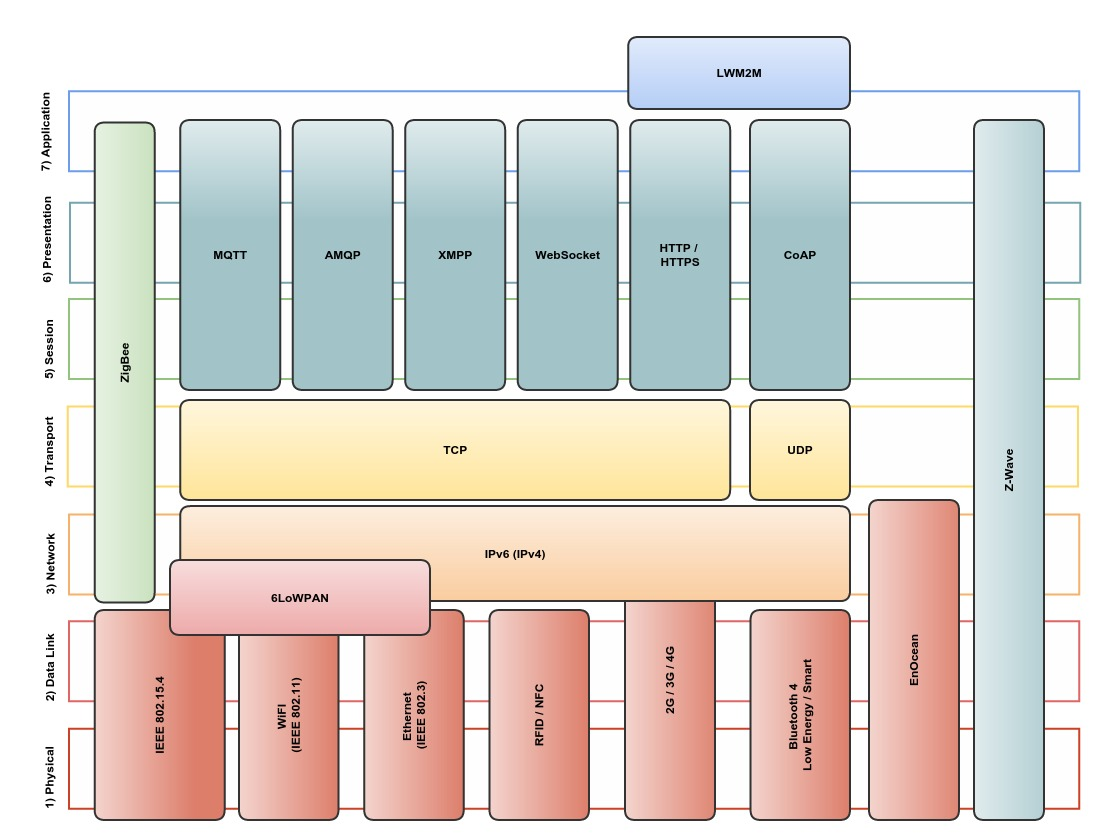
\includegraphics[width=16cm]{./images/IoT-Protokollstack}
  \caption{\gls{acr:IOT}-Protokollstack}
\end{figure}


\subsection{Standards: Kommunikationsprotokolle}
Die ersten Standards für die \gls{acr:IOT}-Welt haben sich im Bereich der Kommunikationsprotokolle entwickelt. Einige dieser Kommunikationsprotokolle wurden spezifisch für das \gls{acr:IOT} entwickelt, andere gibt es schon länger und wurden ursprünglich für einen anderen Zweck entwickelt. Nachfolgend werden die wichtigsten Kommunikationsprotokolle für den Bereich \gls{acr:IOT} beschrieben.


\subsubsection{MQTT}
Das \gls{acr:MQTT} ist ein leichtgewichtiges "`Publish / Subscribe"' Protokoll welches für die Messungen aus der Ferne, Überwachung und Datensammlung eingesetzt wird. Es wird vorwiegend in grossen Netzwerken mit vielen kleinen Geräten eingesetzt, welche überwacht und kontrolliert werden müssen. Die Hauptaufgabe von \gls{acr:MQTT} liegt beim Sammeln von Daten von vielen verschiedenen Endgeräten. \gls{acr:MQTT} hat eine einfache Paket-Struktur und basiert auf \gls{acr:TCPIP}, wodurch sichergestellt wird, dass keine Daten verloren gehen. \gls{acr:MQTT} ist dafür ausgelegt die Daten zu Sammeln und anschliessend an Enterprise Technologien, wie zum Beispiel einen \gls{acr:ESB}, weiterzugeben.

Das Protokoll ist jedoch nicht für die direkte \gls{acr:D2D}-Kommunikation geeignet und arbeitet nicht in Real Time. Die Daten werden mit einer Verzögerung von bis zu mehreren Sekunden übermittelt und verteilt.

Für \gls{acr:MQTT} wird ein zentraler Server, ein sogenannter \gls{acr:MQTT}- oder Message-Broker benötigt. Dieser ist dafür zuständig die eingehenden Nachrichten den interessierten Clients zu verteilen. Die Clients senden dem Message-Broker entweder Daten für ein bestimmtes Thema ("`Topic"') oder registrieren sich für ein bestimmtes Thema, um die übermittelten Daten zu erhalten.



\subsubsection{XMPP}
Das \gls{acr:XMPP} wurde ursprünglich als Protokoll für den Instant Messaging Dienst Jabber entwickelt. \gls{acr:XMPP} ermöglicht eine Text-Kommunikation zwischen "`Punkten"'. Die Kommuunikation erfolgt nicht direkt von Punkt zu Punkt sondern über einen dezentralisierten Server. \gls{acr:XMPP} ist ein offener Standard und somit kann jeder seinen eigenen Server betreiben. Die Stärken von \gls{acr:XMPP} liegen bei der Adressierung, der Sicherheit und der Skalierbarkeit, wobei aktuell noch keine End-To-End Verschlüsselung unterstützt wird. Die Adressierung erfolgt über das Schema \textit{username@domain.com/resource}. Das Protokoll ist ideal für Consumer-Orientierte Anwendungen.

Auch \gls{acr:XMPP} basiert auf \gls{acr:TCPIP}, ist aber auch in der Lage über \gls{acr:HTTP} oder \gls{gls:WebSocket}'s zu kommunizieren. Der Datenaustausch erfolgt in "`near-real-time"', also beinahe Echtzeit.



\subsubsection{AMQP}
Das \gls{acr:AMQP} ist ein binäres transaktionsbasiertes Nachrichten Protokoll, welches für den Einsatz in Nachrichten-orientierter Middleware konzipiert wurde. Es ist in der Lage tausende von zwischengespeicherten Transaktionen ohne Datenverlust zu verarbeiten. Das Protokoll ist darauf ausgelegt keine Daten zu verlieren. Als Basis dient ein zuverlässiges, beziehungsweise im Hinblick auf Daten verlustfreies, Transport-Protokoll wie zum Beispiel \gls{acr:TCPIP} und verschieden definierbare Nachrichtenübermittlungsgarantien. \gls{acr:AMQP} bietet verschiedene Kommunikationsarten wie zum Beispiel "`Publish / Subscribe"', "`Request / Response"' und "`Store and Forward"'. 

Im Gegensatz zu anderen Standardisierungsversuchen im Middleware-Bereich setzt \gls{acr:AMQP} nicht auf dem API-Level, sondern auf dem Wire-Level. Somit wird eine Kommunikation zwischen verschiedenen Middleware-Plattformen ermöglicht.



\subsubsection{HTTP}
Das \gls{acr:HTTP} ist ein auf \gls{acr:TCPIP} zustandsloses Protokoll zur Übermittlung von Daten auf Anwendungsebene. \gls{acr:HTTP} wird im Web praktisch überall eingesetzt und kann sich auch für den Einsatz im \gls{acr:IOT} eigenen.



\subsubsection{WebSocket}
WebSocket ermöglicht eine Voll-Duplex Kommunikation über eine einzelne \gls{acr:TCP}-Verbindung. Das WebSocket Protokoll ermöglicht eine bessere Kommunikation zwischen Browsern und Webseiten / Servern. Jeder der Verbindungsteilnehmer kann jederzeit Daten an den anderen Teilnehmer senden.



\subsubsection{CoAP}
Das \gls{acr:COAP} ist ein leichtgewichtes, binäres Protokoll, welches speziell für kleine, beziehungsweise ressourcenarme  Geräte konzipiert wurde. Semantisch ist \gls{acr:COAP} and \gls{acr:HTTP} ausgerichtet und die Übersetzung von \gls{acr:COAP} nach \gls{acr:HTTP} ist möglich. Wie \gls{acr:HTTP} basiert auch \gls{acr:COAP} auf dem \gls{gls:REST}-Modell. Es können somit Ressourcen unter bestimmten URL's angeboten werden, welche über GET, POST, PUT und DELETE angesprochen werden können. \gls{acr:COAP} zeichnet sich durch seine Einfachheit, Multicasting-Fähigkeit, den geringen Overhead, die Unterstützung von Geräte-Erkennug (Device-Discovery), einen einfachen "`Publish / Subscribe"'-Mechanismus und ein einfaches Caching aus. \gls{acr:COAP} verwendet \gls{acr:UDP} als Transportprotokoll.


\subsubsection{LWM2M}
Das Lightweight \gls{acr:M2M} Protokoll ist ein Device-Management-Standard der Open Mobile Alliance. Das Protokoll selbst basiert auf \gls{acr:COAP} und ist als Client-Server-Protokoll ausgelegt.


\subsection{Standards: Übertragungsprotokolle}
Die Anforderungen der Domäne \gls{acr:IOT} erfordern auch Neuerungen im Bereich der Übertragungsprotokollen und -standards. Nachfolgend werden die wichtigsten Übertragungsprotokolle und -standards für den Bereich \gls{acr:IOT} kurz beschrieben.


\subsubsection{IEEE 802.15.4}
Der Standard IEEE 802.15.4 wurde speziell für den Einsatz auf eingeschränkten Geräten, beziehungsweise eingeschränkten Netzwerken entwickelt und gilt als Schlüsselfaktor für die Etablierung des \gls{acr:IOT}. Dieser drahtlose Standard bildet die Basis für weitere Protokolle und Standards wie ZigBee, WirelessHART oder 6LoWPAN. Der Standard definiert für die Übertragung die Frequenzbänder 868/915 MHz und 2.4 GHz. Es werden Stern und Punkt-zu-Punkt Netzwerke unterstützt.


\subsubsection{ZigBee}
ZigBee ist ein offener Standard für drahtlose Netzwerke, welcher von der ZigBee Alliance entwickelt wird. Die Basis von ZigBee bildet der Standard IEEE 802.15.4. ZigBee ist speziell für \gls{acr:IOT}-Endgeräte ausgelegt und arbeitet daher besonders energieeffizient und ressourcenschonend. Aktuell werden Punkt-zu-Punkt, Stern und Mesh Netzwerk-Topologien unterstützt. Zusätzlich  sind im Funktionsumfang verschlüsselte Verbindungen, Collision-Avoidance und Acknowledgements enthalten. Innerhalb von ZigBee gibt es weitere Standards auf Applikations-Ebene für bestimmte Anwendungsbereiche wie zum Beispiel Home-Automation oder Smart Energy. Die Reichweite des normalen ZigBee Standards im Freien beträgt zwischen 10 und 100 Metern.


\subsubsection{Z-Wave}
Z-Wave ist ein Kommunikationsstandard für die drahtlose Übermittlung von Daten im Bereich der Heimautomation. Er wird von der Firma Sigma Designs in Zusammenarbeit mit der Z-Wave Alliance entwickelt und ist ebenfalls auf einen geringen Energieverbrauch ausgelegt. Der Standard verwendet Frequenzen im Bereich von 850 bis 950 MHz und ist als Mesh-Netzwerk ausgelegt, wobei maximal 4 Hops und maixmal 232 Geräte zugelassen sind. Die Verwaltung des Netzwerkes erfolgt durch einen Primärcontroller. Die Reichweite im freien Gelände beträgt ca. 150 Meter. 

Zusätzlich zum Übertragungsstandard können Z-Wave-Geräte auf Anwendungsebene in verschiedene Klassen eingeteilt werden. Pro Geräteklasse müssen durch den Hersteller bestimmte Pflichtkommandos implementiert werden. neben den Pflichtkommandos kann der Hersteller weitere Funktionalitäten implementieren. Diese müssen jedoch mit dem Z-Wave-Standard konform sein.

\subsubsection{6LoWPAN}
6LoWPAN steht für "`IPv6 over Low Power Wireless Personal Area Networks"' und ist ein auf dem Standard IEEE 802.15.4 basierendes Protokoll zur drahtlosen Datenübermittlung. Es ermöglicht die Übermittlung von IPv6-Packeten über den IEEE 802.15.4 Standard und wurde spezifisch für den Einsatz auf eingeschränkten Geräten entwickelt. 

6LoWPAN kann mit jedem anderen \gls{acr:IP}-Netzwerk (Ethernet oder Wi-Fi), beziungsweise \gls{acr:IP} fähigen Gerät kommunizieren. 

\subsubsection{ANT}
ANT ist ein proprietärer Funkstandard der Firma Dynastream und wurde ursprünglich für die Messung und Überwachung im Bereich Sport und Fitness geschaffen. Mit ANT können drahtlose \gls{acr:PAN}'s gebildet werden. Ebenfalls wird Mesh-Networking unterstützt. Auch ANT verwendet das Frequenzband um 2.4 GHz.


\subsubsection{Bluetooth Smart / Bluetooth Low Energy}
Bluetooth Low Energy (oder auch Bluetooth Smart) ist eine optionale Erweiterung des Bluetooth Standards und ist auf den Einsatz auf eingeschränkten Geräten optimiert. wie auch der normale Bluetooth Standard verwendet Bluetooth Low Energy das 2.4 GHz Frequenzband.


\subsubsection{EnOcean}
EnOcean ist ein Funkstandard der gleichnamigen Firma EnOcean. Das Hauptmerkmal dieser Technologie ist der Fakt, dass auf der Sender-Seite nicht zwingend eine Energie-Quelle vorhanden sein muss. Die zur Übermittlung notwendige Energie wird durch eine physische Interaktion gewonnen (zum Beispiel Betätigung eines Lichtschalters). EnOcean verwendet die Frequenzen 902 MHz, 928.35 MHz und 315 MHz.


\subsubsection{Weitere Standards}
\begin{itemize}
\item DASH7 (Open Source RFID-Standard)
\item ISA100.11a (Drahtloser Netzwerk-Standard der International Society of Automation (ISA), basierend auf IEEE 802.15.4)
\item MiWi (Proprietäres drahtloses Netzwerkprotokoll basierend auf IEEE 802.15.4)
\item WirelessHART (Protokoll für drahtlose Sensor-Netzwerke basierend auf IEEE 802.15.4 und dem \gls{acr:HART})
\item EtherCAT (Ethernet for Control Automation Technology, Echtzeit-Ethernet Protokoll)
\item NFC (Near Field Communication, Standard zum drahtlosen Austausch von Daten über kurze Distanz)
\item RFID (Radio Frequency Identification, Standard zur berührungslosen Identifikation und Lokalisierung )
\item WAMP (Web Application Messaging Protocol, Offener Standard, Subprotokoll des WebSocket Protokoll)
\end{itemize}


\subsection{Frameworks / Erweiterte Protokoll-Stacks}
In diesem Kapitel werden einige Frameworks und Erweiterungen von Protokoll-Stacks vorgestellt. Frameworks vereinfachen die Entwicklung und erlauben einen höheren Abstraktionsgrad in der Anwendung.


\subsubsection{Thread}
Thread ist eine drahtloses Netzwerk-Protokoll welches auf 6LoWPAN und somit auf dem Standard IEEE 802.15.4 und IPv6 basiert. Thread erweitert 6LoWPAN um zusätzliche Funktionalitäten im Bereich Sicherheit, Routing und Setup des Gerätes. Genauere Details zu Thread konnten nicht gefunden werden. Weitere Informationen sind nur über eine kostenpflichtige Mitgliedschaft in der ThreadGroup erhältlich. Thread steht in direkter Konkurrenz zu Iotivity und AllJoyn.


\subsubsection{IoTivity}
IoTivity ist ein Open Source Software Framework des Open Interconnect Consortium (OIC). Ziel von IoTivity ist eine Referenz-Implementation der vom OIC definierten \gls{acr:IOT}-Standards. Das Framework bietet Funktionen zur Device Discovery, Verbindungs- und Ressourcen-Management. Zusätzlich sind folgende Module enthalten:

\begin{itemize}
\item Virtual (Soft) Sensor Manager \\
Aggregierung des Inputs von einem oder mehreren Sensoren und Darstellung als virtuelle Ressource. Die Sensor-Daten können über Queries abgefragt werden.
\item Protocol Plugin Manager\\
Integrationsmöglichkeit für nicht \gls{acr:OIC}-Protokolle.
\item Things Manager\\
Verwaltung von Ressourcen-Gruppen und Ausführen von Gruppen-Aktionen.
\item Ressource Offloading / Notification Manager\\
Verwaltung von Ressourcen für eingeschränkte Geräte.
\item Smart Home Protocol\\
Framework mit Services zur Implementation eines Heimautomations-Controllers.
\end{itemize}

Bei \gls{acr:OIC} Mitglied sind unter anderem Cisco, Intel, Atmel, Honeywell, Dell, Siemens, Acer, Realtek und Hewlett Packard.

\subsubsection{AllJoyn}
AllJoyn ist ein Open Source Framework  der Allseen Alliance. Das Framework bietet Kern-Services zur Erkennung (Discovery) von Geräten und Anwendungen und vereinfacht die Kommunikation und Interaktion mit unbekannten Geräten und Anwendungen. Die Allseen Alliance hat eine grosse Anzahl an Mitgliedern, darunter Canon, Microsoft, Qualcomm, Sony, Cisco, HTC und Lenovo.


\section{Software Testing}
Das Testing, ist wie in allen Domänen, ein essentieller Bestandteil des Software Entwicklungs Prozesses. In dieser Domäne ist das Testing noch wichtiger, da die "`Things"' allenfalls niemals ein Update erhalten (können). "`Things"' werden in grossen Massen hergestellt und auch eingesetzt. Wurden zum Beispiel in einer Öl-Pipeline durch die Wüste mehrere Tausend Sensoren installiert, welche Messwerte und Überwachungsdaten liefern, kann sich die Korrektur eines Fehlers als sehr schwierig herausstellen. Entweder verfügt das Gerät über eine entsprechende Update-Funktionalität und hat eine Verbindung zu einem Back-End System oder der Update erfolgt manuell durch einen technischen Mitarbeiter oder das Gerät wird komplett ausgetauscht. Trotzdem, dass ein Gerät über eine Update-Schnittstelle und eine Verbindung zu einem Netzwerk verfügt, kann es vorkommen, dass ein Update aufgrund mangelnder Hardware-Ressourcen oder zu geringer Bandbreite nicht übertragen oder eingespielt werden kann.

Auch haben Fehler üblicherweise grosse Auswirkungen und sind oft von der Ferne nur schwer festzustellen. Liefern die Sensoren der erwähnten Öl-Pipeline falsche Daten über den Zustand der Leitung, wird gegebenenfalls ein Leck oder ein entstehender Riss nicht rechtzeitig entdeckt, was schlussendlich in einem finanziellen Schaden resultiert.

Dies führt auch bereits zu einem weiteren wichtigen Punkt. "`Things"' und zum Teil auch Gateways können unter verschiedensten physikalischen Bedingungen eingesetzt werden. Bei Servern kann man in der Regel davon ausgehen, dass diese in einem mehr oder weniger gut klimatisierten Rechenzentrum oder einem Server-Raum stehen. Die Bandbreite an physikalischen Einflüssen ist relativ überschaubar. Bei \gls{acr:IOT}-Geräten sieht das etwas anders aus, dort sind die Einflüsse und Bedingungen nur schwer vorhersehbar. Daher haben die meisten Hersteller entsprechende Labor-Umgebungen, wo Hard- und Software unter Extrem- und Ausnahmebedingungen getestet werden.

Nicht nur die Umwelt kann einen Einfluss auf die Geräte haben, sondern auch das verwendete Netzwerk oder die Architektur des Netzwerkes. Auch dafür werden entsprechende Testumgebungen benötigt. Zusätzlich muss die Interaktion mit unbekannten Drittgeräten getestet werden.

Der Funktionsumfang der \gls{acr:IOT}-Endgeräte ist in der Regel sehr überschaubar und die Funktionalitäten weisen eine geringe Komplexität auf. Dadurch wird der Test der eigentlichen Funktionalität etwas vereinfacht, was aber durch die bereits oben erwähnten Punkte mehr als kompensiert wird.


Für Gateways und Back-End Systeme wird für das Software Testing analog der Standard-Domäne verfahren. Bei den Gateways ist zusätzlich sicherzustellen, dass diese über die korrekten Versionen der eingesetzten Kommunikationsstacks verfügen. Ist dies nicht der Fall, können die \gls{acr:IOT}-Endgeräte unter Umständen nicht mehr mit dem Gateway kommunizieren.


\section{Software Maintenance}
Die Maintenance von Software welche für \gls{acr:IOT}-Endgeräte entwickelt wurde ist schwierig, beziehungsweise aufwändig. Wie bereits im vorangehenden Kapitel aufgezeigt, kann die Software auf \gls{acr:IOT}-Endgeräte schwierig zum updaten sein. Ist ein entsprechender Update-Mechanismus vorhanden, ist ein besonders Augenmerk auf den Rollout zu legen, da schnell mehrere 10'000 Geräte betroffen sein können. Hier stellen sich Fragen wie: Wann wird das Update eingespielt? Welche Geräte erhalten das Update in welcher Reihenfolge? Was sind die Auswirkungen während / nach dem Update? Wie werden die Besitzer der Geräte informiert? Gibt es Abhängigkeiten zwischen verschiedenen Software-Versionen? Gibt es Abhängigkeiten zwischen Endgerät, Gateway und Back-End System?

Unter Umständen können gewisse Geräte nicht aktualisiert werden. Daher muss sichergestellt werden dass das Gateway und gegebenenfalls auch das Back-End System rückwärts kompatibel bleiben. Durch ein vorausschauendes und gutes Schnittstellendesign kann diese Situation umgangen oder entschärft werden.



\section{Software Configuration Management}
Um ein Software-Update erfolgreich auszurollen ist das Configuration Management sehr wichtig. Zuerst muss der Update-Prozess in einer Testumgebung für die sich im Betrieb befindlichen Geräte getestet werden. Dafür müssen Informationen bezüglich eingesetzten Versionen von Hard- und Software aus dem Configuration Management herangezogen werden. Sind sämtliche Tests gut verlaufen kann der entsprechende Update ausgerollt und nach und nach die dazugehörigen Configuration Items aktualisiert werden.



\section{Software Engineering Management}
Das Software Engineering Management entspricht grundsätzlich dem Vorgehen in der Standard-Domäne. Es müssen jedoch allen Beteiligten die Eigen- und Besonderheiten dieser Domäne bekannt sein. Besonderes Gewicht ist dem Risk und Quality Management beizumessen.



\section{Software Engineering Process}
Der Software Entwicklungsprozess von \gls{acr:IOT}-Anwendungen ist je nach Element unterschiedlich. Die Entwicklungszeitraum für ein "`Things"' ist relativ kurz, wobei für die Implementation viele verschiedene Fähigkeiten erforderlich sind. Im Gegensatz dazu ist der Entwicklungsprozess von Gateways und Back-End Systemen aufwändiger und entspricht eher dem Entwicklungsprozess von Systemen in der Standard-Domäne.



\section{Software Engineering Tools and Methods}
Die eingesetzten Tools und Methoden sind wiederum vom betroffenen Element abhängig. Bei "`Things"' kommen Werkzeuge und Methoden zum Einsatz, welche sich besonders für die Entwicklung und das Testing von Embedded Systems eignen. Allenfalls müssen sogar eigene Tools entwickelt werden, um den Software Entwicklungsprozess und das Testing optimal zu unterstützen. Denkbar wäre hier zum Beispiel eine Simulationsanlage zum automatisierten Testen der Geräte unter verschiedenen physikalischen Bedingungen und Umwelteinflüssen. Als Programmiermethoden kommen eher strukturierte, objektorientierte oder spezifische (zum Beispiel bei Real-Time Anwendungen / Betriebssystemen) Methoden zur Anwendung.

Die Entwicklung der Gateways und Back-End Systeme bedient sich im grossen und ganzen der Werkzeuge und Methodiken der Standard- und Big-Data Domäne. 


\section{Software Quality}
Die Software Qualität ist im Bereich \gls{acr:IOT} extrem wichtig, insbesondere im Bereich der "`Things"'. Da das Ziel der klassischen Softwareentwicklung ebenfalls ein hohe Qualität ist, gibt es auch hier grundsätzlich keinen Unterschied im Rahmen der Software Entwicklung.


\section{Verwandte Disziplinen}
Es gibt einige weitere Disziplinen, welche aufgrund der starken Innovationskraft einen grossen Einfluss auf die Domäne "`Internet of Things"' und das Software Egineering in dieser Domäne haben. Dies sind unter anderem das Computer Engineering, Computer Science, Mathematik und System Engineering.
